\documentclass[a4paper,11pt]{article}

\usepackage{amsmath}
\usepackage[pdftex]{graphicx}

\usepackage[english,greek]{babel}

\usepackage{lmodern}

\usepackage{listings}

\lstset{
  basicstyle=\ttfamily,
  columns=fullflexible,
  frame=single,
  breaklines=true
}

% Αφαίρεσε (Εισήγαγε) την παρακάτω γραμμή σε σχόλιο αν ο επεξεργαστής κειμένου (δεν) χρησιμοποιεί κωδικοποίηση Unicode για Ελληνικά
\usepackage[utf8x]{inputenc}

% Αφαίρεσε (Εισήγαγε) την παρακάτω γραμμή σε σχόλιο αν ο επεξεργαστής κειμένου (δεν) χρησιμοποιεί κωδικοποίηση iso-8859-7 για Ελληνικά
%\usepackage[iso-8859-7]{inputenc}

%Δημιουργία συντομεύσεων για αλλαγή γραφής σε Ελληνικά/Αγγλικά
\newcommand{\lt}{\latintext}
\newcommand{\gt}{\greektext}

\title{1η Υποχρεωτική Εργασία \\ Στο Μάθημα της Αριθμητικής Ανάλυσης: \\ Άσκηση 1}
\author{Όνοματεπώνυμο: Μπαρακλιλής Ιωάννης  \\  ΑΕΜ: 3685}
\date{16 Δεκεμβρίου 2020}

\begin{document}

\maketitle

\section{Αρχική Ανάλυση της συνάρτησης \lt $f(x)$}

Η συνάρτηση που δόθηκε είναι η $f(x) = e^{sin^{3}x} + x^6 − 2x^4 − x^3 − 1$ με πεδίο ορισμού το $[-2,2]$ με γραφική παράσταση:\\
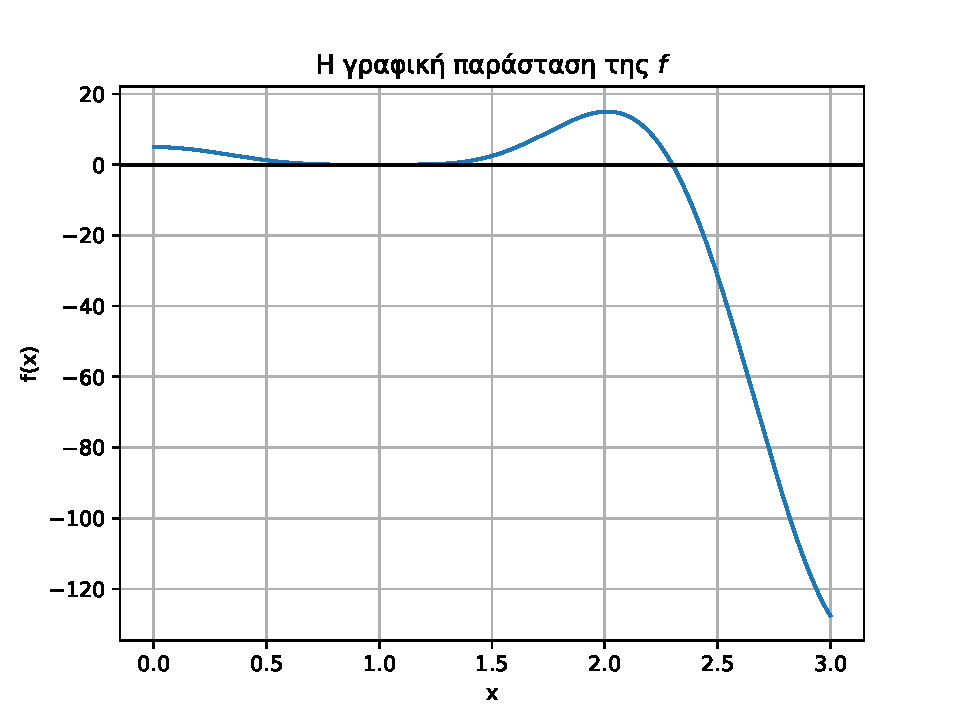
\includegraphics[width=\linewidth]{Exercise1/f_figure.pdf}\\
Ζητείται να βρεθούν όλες οι ρίζες της με ακρίβεια 5ου δεκαδικού ψηφίου.\\
\par
Απο την γραφική παράσταση μπορούμε να παρατηρήσουμε 3 ρίζες:\\
\begin{itemize}
    \item Μία κοντά στο $-1.0$ στο διάστημα $[-1.5, -1.0]$,
    \item μία κοντά στο $1.5$ στο διάστημα $[1.25, 1.75]$ και
    \item μία κοντά στο $0.0$.
\end{itemize}
Για τα δύο πρώτα διαστήματα μπορούμε να επαληθεύσουμε την ύπαρξη των ριζών με το θεώρημα {\lt Bolzano}: Η συνάρτηση $f$ είναι συνεχής στα διαστήματα $[-1.5, -1.0]$ και $[1.25, 1.75]$ και ισχύει $f(-1.5) \cdot f(-1.0) \simeq 4.01127 \cdot -0.44889 < 0$ και
$f(1.25) \cdot f(1.75) \simeq -1.67073 \cdot 6.19847 < 0$. Οπότε σύμφωνα με το θεώρημα {\lt Bolzano} υπάρχει μία ρίζα σε κάθε ένα απο τα διαστήματα $[-1.5, -1.0]$ και $[1.25, 1.75]$.\\

Για την ρίζα κοντα στο $0.0$ δεν μπορούμε να ορίσουμε διάστημα κοντά σε αυτό διότι όπως φαίνεται και στην γραφική παράσταση η $f$ είναι αρνητική αμέσως μετά την ρίζα στο $[-1.5, -1.0]$ μέχρι και την ρίζα στο $[1.25, 1.75]$. Παρ' όλα αυτά, μπορούμε με μία απλή αντικατάσταση να δείξουμε ότι $f(0) = 0$ : $f(0) = e^{sin^{3}0} + 0^6 - 2 \cdot 0 - 0^3 - 1 = e^0 + 0 - 0 - 0 - 1 = 1 - 1 = 0$.


Άρα εφόσον βρήκαμε τα διαστήματα στα οποία υπάρχουν οι ρίζες, αρκεί να χρησιμοποιήσουμε τις επαναληπτικές μεθόδους για να τις βρούμε.

\section{Ερώτημα (α): Η μέθοδος διχοτόμισης}
Στην μέθοδο της διχοτόμισης αρχικά ορίζω ένα διάστημα στο οποίο γνωρίζω ότι υπάρχει μία ρίζα και το χωρίζω σε δύο ίσα διαστήματα και επαναλαμβάνω αυτή την μέθοδο θεωρώντας ως διάστημα που χωρίζω αυτό το διάστημα με ένα άκρο το μέσο (έστω {\lt m}) του προηγουμένου και άλλο άκρο το άκρο του προηγουμένου (έστω {\lt e}) για το οποίο ισχύει $f(m) \cdot f(e) < 0$ μέχρις ότου το μισό του πλάτους του νέου διαστήματος να είναι μικρότερο απο την απαιτούμενη ακρίβεια, καθώς γνωρίζουμε ότι η ρίζα βρίσκεται στο διάστημα και είναι είτε το μέσο του διαστήματος είτε βρίσκεται ανάμεσα στο μέσο και ένα άκρο αυτού.

\gt Η μέθοδος διχοτόμισης υλοποιείται προγραμματιστικά στην γλώσσα {\lt python} (3.7) στο αρχείο {\lt a\textunderscore Bisection.py} το οποίο φαίνεται παρακάτω:

\lt
\lstinputlisting[language=Python]{a_Bisection.py}
\gt

Στον παραπάνω κώδικα:
\\
Αρχικά, ορίζω την συνάρτηση {\lt f} που υλοποιεί την $f$.\\
\\
Στην συνέχεια, ορίζω την συνάρτηση {\lt bisection} η οποία δέχεται την συνάρτηση, το αριστερό άκρο του αρχικού διαστήματος, το δεξί άκρο του αρχικού διαστήματος και τα ζητούμενα ψηφία ακρίβειας:\par
Αρχικά, ορίζω ψευδώνυμα για την συνάρτηση, αρχή και τέλος διαστήματος αναζήτησης ρίζας (με ονόματα {\lt f, a, b} αντίστοιχα).
Ακόμη, ορίζω και αρχικοποιώ την μεταβλητή {\lt iteration\textunderscore counter}, σε 0,  που <<μετράει>> τις επαναλήψεις της μεθόδου.
Επίσης, ορίζω και δίνω τιμές στις μεταβλητές που αποθηκεύουν την τιμή συνάρτησης στην αρχή και τέλος διαστήματος, το μέσο του διαστήματος και την τιμή συνάρτησης στο μέσο του διαστήματος (με ονόματα {\lt fa, fb, m, fm} αντίστοιχα). 

Στην συνέχεια, αρχίζει ατέρμονος βρόχος (που θα τερματισει αργότερα όταν <<πετύχω>> την επιθυμιτή ακρίβεια) όπου γίνονται οι ενέργειες:\\
Πρώτα, ελέγχω αν η τρέχουσα εκτίμηση (μέσο του διαστήματος) αποτελεί ρίζα της συνάρτησης, επειδή αν ισχύει αυτό δεν χρειάζεται να συνεχίσω την αναζήτηση γιατί βρέθηκε η ζητούμενη ρίζα. Άν είναι, τερματίζω την εκτέλεση της συνάρτησης και επιστρέφω την εκτίμηση της ρίζας και τον αριθμό των επαναλήψεων που χρειάστηκαν για να βρεθεί.\\
Στην συνέχεια (η τρέχουσα εκτίμιση δεν αποτελεί ρίζα), υπολογίζω το νέο διάστημα αναζήτησης: Άν το γινόμενο της συνάρτησης στο αριστερό άκρο ({\lt a}) με την συνάρτηση στο μέσο του διαστήματος ({\lt m}) είναι αρνητικό ({\lt $fa * fm < 0$}) τότε έχω ρίζα στο διάστημα $[a, m]$ και ορίζω νέο διάστημα αναζήτησης ορίζοντας ως νέο δεξί άκρο διαστήματος το μέσο του παλιού (θέτω {\lt b = m} και για να μην το ξαναυπολογίσω θέτω {\lt fb = fm}). Διαφορετικά (το πάνω γινόμενο είναι θετικό), έχω ρίζα στο διάστημα {\lt $[m, b]$} (όπου {\lt b} δεξί άκρο του αρχικού διαστήματος) και ορίζω νέο διάστημα αναζήτησης ορίζοντας ως νέο αριστερό άκρο διαστήματος το μέσο του παλιού (θέτω {\lt a = m} και για να μην το ξαναυπολογίσω θέτω {\lt fa = fm}).\\
Μετά, ενημερώνω την μεταβλητή που αποθηκεύει τον αριθμό των επαναλήψεων και εκείνη που αποθηκεύει την παλιά τιμή του μέσου που θα χρησιμοποιήσω αργότερα για τον έλεγχο του σφάλματος, υπολογίζω την νέα εκτίμηση ρίζας και υπολογίζω την τιμή της συνάρτησης σε αυτή την εκτίμηση.\\
Τέλος, ελέγχω άν η διαφορά της νέας και παλιάς εκτίμησης είναι μικρότερη του ανεκτού σφάλματος (γνωρίζω ότι η μέθοδος συγκλίνει οπότε ελέγχω με αυτόν τον τρόπο την ακρίβεια εκτίμησης) και αν είναι επιστρέφω την εκτίμηση της ρίζας και τον αριθμό των επαναλήψεων που χρειάστηκαν για να βρεθεί (τερματίζοντας την εκτέλεση της συνάρτησης).

Επίσης, στο τμήμα του κώδικα που εκτελείται όταν τρέχουμε το αρχείο (μετά τον ορισμό των συναρτήσεων) εκτελώ την συνάρτηση {\lt bisection}, με παραμέτρους την συνάρτηση $f$ που ορίστηκε πιο πάνω, την αρχή και το τέλος του αντίστοιχου διαστήματος και τον αριθμό των δεκαδικών ψηφίων ακρίβειας της εκτίμησης ρίζας που πρέπει να <<πετύχει>> η συνάρτηση (που είναι 5 λόγω της εκφώνησης), για κάθε διάστημα στο οποίο υπάρχει ρίζα και αποθηκεύω στις μεταβλητές {\lt root, loops\textunderscore counter} τα αποτελέσματα της συνάρτησης, που είναι η εκτίμηση της ρίζας και ο αριθμός επαναλήψεων που χρειάστηκαν για να επιτευχθεί αυτή η ακρίβεια, πρίν τα τυπώσω με μία {\lt print}.

\par
\vspace{20pt}

Άν τρέξουμε τον κώδικα, θα τυπωθεί το ακόλουθο:\\

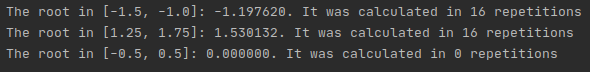
\includegraphics[width=\linewidth]{Exercise1/run_Bisection.png}\\

Άρα, διαπιστώνουμε ότι η συνάρτηση έχει τις ρίζες: -1.197620 (που βρήκε σε 16 επαναλήψεις) και 1.530132 (που βρήκε σε 16 επαναλήψεις). Διαπιστώνουμε ότι βρήκε και τις δύο ρίζες στον ίδιο αριθμό επαναλήψεων.\\
Επίσης, πρίν δείχθηκε ότι άλλη μία ρίζα είναι το 0, για την οποία δεν μπορούμε να εφαρμόσουμε μέθοδο διχοτόμισης διότι δεν πληρούνται οι προυποθέσεις του θεωρήματος {\lt Bolzano} για διάστημα που μοναδική ρίζα το $x = 0$.\\
Παρ'' όλα αυτά, με την τρίτη κλήση της συνάρτησης {\lt bisection} στο διάστημα $[-0.5, 0.5]$ η συνάρτηση βρίσκει την ρίζα σε 0 επαναλήψεις.\\
Αυτο συμβαίνει γιατί με τον τρόπο με τον οποίο έχει δομηθεί η συνάρτηση {\lt bisection} κατά την πρώτη επανάληψη ελέγχει αν το μέσο του διαστήματος είναι ρίζα οπότε εφόσον το άθροισμα των τιμών των δύο άκρων του διαστήματος είναι 0 τότε το μέσο τους είναι το 0, το οποίο τυχαίνει να είναι ρίζα.

\section{Ερώτημα (β): H μέθοδος {\lt Newton-Raphson}}
\par
Στην μέθοδο {\lt Newton-Raphson} για να βρεθεί προσέγγιση της ρίζας χρησιμοποιούμε την ακολουθία 
\[x_n = x_{n-1} - \dfrac{f(x_{n-1})}{f'(x_{n-1})} \] 
για να βρούμε την επόμενη εκτίμηση ρίζας. Ορίζουμε εμείς αρχικό σημείο $x_0$ να είναι τέτοιο ώστε $f(x_0) \cdot f''(x_0) > 0$. Έτσι (σύμφωνα με την θεωρία), η μέθοδος θα συγκλίνει τετραγωνικά προς την πραγματική ρίζα.\\

Επομένως, πρέπει να υπολογίσουμε την πρώτη και δεύτερη παράγωγο της $f$:

\par
\vspace{20pt}
\begin{itemize}
    \item Η $f$ είναι παραγωγίσιμη με $f'(x) = 3sin^2(x) \cdot cos(x) \cdot e^{sin^3x} + 6x^5 - 8x^3 - 3x^2$ και 
    \item Η $f'$ είναι παραγωγίσιμη με $f''(x) = 9cos^2x \cdot sin^4x \cdot e^{sin^3x} - 3sin^3x \cdot e^{sin^3x} + 6sinx \cdot cos^2x \cdot e^{sin^3x} + 30x^4 - 24x^2 - 6x$.
\end{itemize}

Απο την γραφική παράσταση στο μέρος της αρχικής ανάλυσης της συνάρτησης, παρατηρούμε ότι υπάρχουν ρίζες κοντά στα σημεία -1.5, 1.75 και 0. Μπορούμε να πάρουμε αυτά τα σημεία ως αρχικές εκτιμήσεις ριζών αρκεί να ικανοποιούν τον παραπάνω περιορισμό.\\
Έχουμε λοιπόν:
Για το σημείο $x = -1.5$: $f(-1.5) \cdot f''(-1.5) \simeq 4.011 \cdot 107.98 > 0$ άρα συγκλίνει σε αυτό.\\
Για το σημείο $x = 1.75$: $f(1.75) \cdot f''(1.75) \simeq 6.20 \cdot 191.14 > 0$ άρα συγκλίνει σε αυτό.\\
Για το σημείο $x = 0$: $f(0) \cdot f''(0) = 0 \cdot 0 = 0$! Στο πρώτο μέρος έχει αποδειχθεί ότι $f(0) = 0 $ που σε συνδυασμό με το προηγούμενο σημαίνουν ότι η $f$ έχει ρίζα στο $x = 0$ στην οποία η προσέγγιση με {\lt Newton-Raphson} δεν συγκλίνει τετραγωνικά αλλά γραμμικά (επειδή  $f'(0) = 0$). Για αρχικό σημείο θα πάρουμε το $x = 0.1$ που είναι κοντά στο 0 (δεν παίρνουμε $x = 0$ γιατί $f'(0) = 0$).\\

Η μέθοδος {\lt Newton-Raphson} υλοποιείται προγραμματιστικά στην γλώσσα {\lt python} στο αρχείο {\lt b\textunderscore Newton\textunderscore Raphson.py} το οποίο φαίνεται παρακάτω:

\lt
\lstinputlisting[language=Python]{b_Newton_Raphson.py}
\gt

Στον παραπάνω κώδικα:
\\
Αρχικά, ορίζω τις συναρτήσεις {\lt f, f\textunderscore derivative} που υλοποιούν την συνάρτηση $f(x)$ και την συνάρτηση $f'(x)$ αντίστοιχα.\\
\\
Στην συνέχεια, ορίζω την συνάρτηση {\lt newton\textunderscore raphson} η οποία δέχεται την συνάρτηση, την παράγωγο της συνάρτησης, το αρχικό σημείο της ακολουθίας και τα ζητούμενα ψηφία ακρίβειας:\par
Αρχικά, ορίζω ψευδώνυμα για την συνάρτηση και την παράγωγο της (με ονόματα {\lt f} και {\lt f\textunderscore d} αντίστοιχα).
Επίσης, ορίζω και αρχικοποιώ την μεταβλητή {\lt iteration\textunderscore counter}, σε 0,  που <<μετράει>> τις επαναλήψεις της μεθόδου και την μεταβλητή {\lt x}, στο αρχικό σημείο της ακολουθίας (που δίνεται ως όρισμα), που αποθηκεύει την τρέχουσα εκτίμηση της ρίζας.

Στην συνέχεια, αρχίζει ατέρμονος βρόχος (που θα τερματισει αργότερα όταν <<πετύχω>> την επιθυμιτή ακρίβεια) όπου γίνονται οι ενέργειες:\\
Πρώτα, ελέγχω αν η τρέχουσα εκτίμηση αποτελεί ρίζα της συνάρτησης, επειδή αν ισχύει αυτό δεν χρειάζεται να συνεχίσω την αναζήτηση γιατί βρέθηκε η ζητούμενη ρίζα. Άν είναι τερματίζω την εκτέλεση της συνάρτησης και επιστρέφω την εκτίμηση της ρίζας και τον αριθμό των επαναλήψεων που χρειάστηκαν για να βρεθεί.\\
Στην συνέχεια (η τρέχουσα εκτίμιση δεν αποτελεί ρίζα): ενημερώνω την μεταβλητή που αποθηκεύει τον αριθμό των επαναλήψεων, υπολογίζω το επόμενο στοιχείο ακολουθίας που αποτελεί την επόμενη εκτίμηση της ρίζας ($x_n = x_{n-1} - \dfrac{f(x_{n-1})}{f'(x_{n-1})}$) και το αποθηκεύω στην (νέα) μεταβλητή {\lt x\textunderscore next}.\\
Τέλος, ελέγχω άν η διαφορά της νέας και παλιάς εκτίμησης (διαφορά μεταβλητών {\lt x} και {\lt x\textunderscore next} είναι μικρότερη του ανεκτού σφάλματος (γνωρίζω ότι η μέθοδος συγκλίνει οπότε ελέγχω με αυτόν τον τρόπο την ακρίβεια εκτίμησης) και άν είναι επιστρέφω την εκτίμηση της ρίζας και τον αριθμό των επαναλήψεων που χρειάστηκαν για να βρεθεί (τερματίζοντας την εκτέλεση της συνάρτησης).\\

Επίσης, στο τμήμα του κώδικα που εκτελείται όταν τρέχουμε το αρχείο (μετά τον ορισμό των συναρτήσεων) εκτελώ την συνάρτηση {\lt newton\textunderscore raphson}, με παραμέτρους τις συναρτήσεις {\lt f} και {\lt f\textunderscore derivative} που ορίστηκαν πιο πάνω, το αρχικό σημείο της ακολουθίας και τον αριθμό των δεκαδικών ψηφίων ακρίβειας της εκτίμησης ρίζας που πρέπει να <<πετύχει>> η συνάρτηση (που είναι 5 λόγω της εκφώνησης), για κάθε σημείο <<κοντά>> στο οποίο υπάρχει ρίζα και αποθηκεύω στις μεταβλητές {\lt root, loops\textunderscore counter} τα αποτελέσματα της συνάρτησης, που είναι η εκτίμηση της ρίζας και ο αριθμός επαναλήψεων που χρειάστηκαν για να επιτευχθεί αυτή η ακρίβεια, πρίν τα τυπώσω με μία {\lt print}.

Άν τρέξουμε τον κώδικα, θα τυπωθεί το ακόλουθο:\\

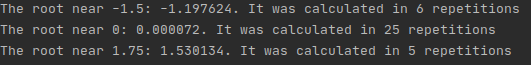
\includegraphics[width=\linewidth]{Exercise1/run_Newton_Raphson.png}\\

Άρα, διαπιστώνουμε ότι η συνάρτηση έχει τις ρίζες: -1.197624 (που βρήκε σε 6 επαναλήψεις), 0.000072 (που βρήκε σε 25 επαναλήψεις) και 1.530134 (που βρήκε σε 5 επαναλήψεις). Διαπιστώνουμε ότι βρήκε δύο απο τις ρίζες στον ίδιο περίπου αριθμό επαναλήψεων, όμως η ρίζα κοντά στο 0 βρέθηκε σε σημαντικά μεγαλύτερο αριθμό επαναλήψεων.\\

Εφόσον έχουν βρεθεί οι ρίζες, μπορεί να συζητηθεί το για ποιες ρίζες συγκλίνει τετραγωνικά και για ποιες όχι.
Η μέθοδος για να συγκλίνει τετραγωνικά για μία ρίζα $x = x^*$ πρέπει $f$ να είναι δύο φορές συνεχώς παραγωγίσιμη σε μία περιοχή του {\lt $x^*$} και η {\lt $x^*$} να είναι απλή ρίζα της $f(x) = 0$, σε διαφορετική περίπτωση συγκλίνει γραμμικά σε αυτή την ρίζα.
Έχουμε οτι $f$ και $f'$ συνεχείς και παραγωγίσιμες στο πεδίο ορισμού τους (επομένως και σε περιοχή του εκάστοτε {\lt $x^*$} και:
\begin{itemize}
    \item Για $x = -1.197624$: $f(-1.197624) = 0.000001 \simeq 0$ και $f'(-1.197624) \simeq -4.92 \neq 0$ (δηλαδή {\lt $x$} είναι απλή ρίζα της $f(x) = 0$).
    \item Για $x = 1.530134$: $f(1.530134) = 0.000007 \simeq 0$ και $f'(1.530134) \simeq 14.97 \neq 0$ (δηλαδή {\lt $x$} είναι απλή ρίζα της $f(x) = 0$).
    \item Για $x = 0.000072$: $f(0.000072) = 0.000000 = 0$ και $f'(0.000072) = 0.000000 = 0$ (δηλαδή {\lt $x$} δεν είναι απλή ρίζα της $f(x) = 0$).
\end{itemize}

Απο τα παραπάνω διαπιστώνουμε ότι συγκλίνουν τετραγωνικά οι ρίζες -1.197624 και 1.530134.\\
Η ρίζα 0.000072 δεν συγκλίνει τετραγωνικά αλλά γραμμικά.

\par
Σχετικά με το χαρακτηριστικό των ριζών για τις οποίες η μέθοδος {\lt Newton-Raphson} δεν συγκλίνει τετραγωνικά, γνωρίζουμε ότι δεν συγκλίνουν τετραγωνικά οι ρίζες οι οποίες δεν είναι απλές, αυτές δηλαδή που έχουν πολλαπλότητα μεγαλύτερη απο 1.\\
Αποδείχθηκε παραπάνω ότι $f(0) = f'(0) = f''(0) = 0$.
Επιπλέον, αν παραγωγίσουμε την $f''$ εχουμε την $f^{(3)}(x) = 27cos^3x \cdot sin^6x \cdot e^{sin^3x} - 27cosx \cdot sin^5x \cdot e^{sin^3x} + 54cos^3x \cdot sin^3x \cdot e^{sin^3x} - 21cosx \cdot sin^2x \cdot e^{sin^3x} + 6cos^3x \cdot e^{sin^3x} + 120x^3 -48x -6$.\\
Έχω $f^{(3)}(0) = 0$.\\

Τέλος, αν παραγωγίσουμε την $f^{(3)}$ έχουμε την $f^{(4)} = 81cos^4x \cdot sin^8x \cdot e^{sin^3x} - 162cos^2x \cdot sin^7x \cdot e^{sin^3x} + 27e^{sin^3x} \cdot sin^6x + 324cos^4x \cdot sin^5x \cdot e^{sin^3x} -360cos^2x \cdot sin^4x \cdot e^{sin^3x} + 21e^{sin^3x} \cdot sin^3x + 180sin^2x \cdot cos^4x \cdot e^{sin^3x} - 60sinx \cdot cos^2x \cdot e^{sin^3x} + 360x^2 - 48$.\\
Έχω $f^{(4)}(0) = -48 \neq 0$.\\
Δηλαδή $f(0) = f'(0) = f''(0) = f^{(3)}(0) = 0$ και $f^{(4)}(0) \neq 0$ οπότε η ρίζα $x = 0$ είναι ρίζα πολλαπλότητας 4, που εξηγεί το γεγονός μη τετραγωνικής σύγκλισης.

\section{Ερώτημα (γ): H μέθοδος της τέμνουσας}

Στην μέθοδο της τέμνουσας για να βρεθεί η προσέγγιση της ρίζας χρησιμοποιούμε την ακολουθία
\[ x_n = x_{n-1} - \dfrac{f(x_{n-1}) \cdot (x_{n-1} - x_{n-2})}{f(x_{n-1}) - f(x_{n-2})} \]
για να βρούμε την επόμενη εκτίμηση ρίζας. Ορίζουμε ως $x_1$, $x_0$ ως τα άκρα του διαστήματος στο οποίο αναζητούμε ρίζα.\\

Απο την ανάλυση της συνάρτησης γνωρίζουμε ότι η συνάρτηση $f$ έχει τρείς ρίζες: Μία στο διάστημα $[-1.5, -1.0]$, $[1.25, 1.75]$ και μία κοντά στο $0.0$ όπου ορίζουμε διάστημα $[-0.5, 0.5]$.

Η μέθοδος της τέμνουσας υλοποιείται προγραμματιστικά στην γλώσσα {\lt python} στο αρχείο {\lt c\textunderscore Secant.py} το οποίο φαίνεται παρακάτω:

\lt
\lstinputlisting[language=Python]{c_Secant.py}
\gt

Στον παραπάνω κώδικα:
\\
Αρχικά, ορίζω την συνάρτηση {\lt f} που υλοποιεί την $f$.\\
\\
Στην συνέχεια, ορίζω την συνάρτηση {\lt secant} η οποία δέχεται την συνάρτηση, τα δύο αρχικά σημεία και τα ζητούμενα ψηφία ακρίβειας:\par
Αρχικά, ορίζω ψευδώνυμο για την συνάρτηση (με όνομα {\lt f}), ορίζω και αρχικοποιώ την μεταβλητή {\lt iteration\textunderscore counter}, σε 0,  που <<μετράει>> τις επαναλήψεις της μεθόδου και ορίζω και αρχικοποιώ τις μεταβλητές {\lt x1} και {\lt x2}, που αποθηκεύουν την παλιά και καινούρια αντίστοιχα εκτίμηση της ρίζας, στις τιμές αρχικών σημείων {\lt point\textunderscore one} και {\lt point\textunderscore two} αντίστοιχα που δίνοται ως ορίσματα.

Στην συνέχεια, αρχίζει ατέρμονος βρόχος (που θα τερματισει αργότερα όταν <<πετύχω>> την επιθυμιτή ακρίβεια) όπου γίνονται οι ενέργειες:\\
Πρώτα, ελέγχω αν η τρέχουσα εκτίμηση αποτελεί ρίζα της συνάρτησης, επειδή αν ισχύει αυτό δεν χρειάζεται να συνεχίσω την αναζήτηση γιατί βρέθηκε η ζητούμενη ρίζα. Άν είναι τερματίζω την εκτέλεση της συνάρτησης και επιστρέφω την εκτίμηση της ρίζας και τον αριθμό των επαναλήψεων που χρειάστηκαν για να βρεθεί.\\
Στην συνέχεια (η τρέχουσα εκτίμιση δεν αποτελεί ρίζα): ενημερώνω την μεταβλητή που αποθηκεύει τον αριθμό των επαναλήψεων, υπολογίζω το επόμενο στοιχείο ακολουθίας που αποτελεί την επόμενη εκτίμηση της ρίζας ($x_n = x_{n-1} - \dfrac{f(x_{n-1}) \cdot (x_{n-1} - x_{n-2})}{f(x_{n-1}) - f(x_{n-2})}$) και το αποθηκεύω στην (νέα) μεταβλητή {\lt x\textunderscore next}.\\
Τέλος, ελέγχω άν η διαφορά της νέας και παλιάς εκτίμησης (διαφορά μεταβλητών {\lt x2} και {\lt x\textunderscore next} είναι μικρότερη του ανεκτού σφάλματος (γνωρίζω ότι η μέθοδος συγκλίνει οπότε ελέγχω με αυτόν τον τρόπο την ακρίβεια εκτίμησης) και άν είναι επιστρέφω την εκτίμηση της ρίζας και τον αριθμό των επαναλήψεων που χρειάστηκαν για να βρεθεί (τερματίζοντας την εκτέλεση της συνάρτησης). 
Διαφορετικά (η διαφορά μεταβλητών {\lt x2} και {\lt x\textunderscore next} δεν είναι μικρότερη του ανεκτού σφάλματος), ενημερώνω τις μεταβλητές {\lt x1} και {\lt x2} (το {\lt x1} παίρνει την τιμή του {\lt x2} και το {\lt x2} παίρνει την τιμή του {\lt x\textunderscore next}).\\
Επίσης, στο τμήμα του κώδικα που εκτελείται όταν τρέχουμε το αρχείο (μετά τον ορισμό των συναρτήσεων) εκτελώ την συνάρτηση {\lt secant}, με παραμέτρους τις συναρτήσεις {\lt f}, τα άκρα του διαστήματος και τον αριθμό των δεκαδικών ψηφίων ακρίβειας της εκτίμησης ρίζας που πρέπει να <<πετύχει>> η συνάρτηση (που είναι 5 λόγω της εκφώνησης), για κάθε διάστημα στο οποίο υπάρχει ρίζα και αποθηκεύω στις μεταβλητές {\lt root, loops\textunderscore counter} τα αποτελέσματα της συνάρτησης, που είναι η εκτίμηση της ρίζας και ο αριθμός επαναλήψεων που χρειάστηκαν για να επιτευχθεί αυτή η ακρίβεια, πρίν τα τυπώσω με μία {\lt print}.

Άν τρέξουμε τον κώδικα, θα τυπωθεί το ακόλουθο:\\

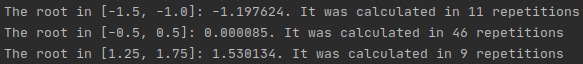
\includegraphics[width=\linewidth]{Exercise1/run_Secant.png}\\

Άρα, διαπιστώνουμε ότι η συνάρτηση έχει τις ρίζες: -1.197624 (που βρήκε σε 11 επαναλήψεις), 0.000085 (που βρήκε σε 46 επαναλήψεις) και 1.530134 (που βρήκε σε 9 επαναλήψεις). Διαπιστώνουμε ότι βρήκε δύο απο τις ρίζες στον ίδιο περίπου αριθμό επαναλήψεων, όμως η ρίζα κοντά στο 0 βρέθηκε σε σημαντικά μεγαλύτερο αριθμό επαναλήψεων.

\section*{Συμπέρασμα}

Τέλος, πρέπει να σχολιαστεί η διαφορά ταχύτητας σύκγλισης των τριών παραπάνω μεθόδων. Παρατηρούμε ότι, εν γένει, η μέθοδος {\lt Newton-Raphson} είναι η ταχύτερη απο τις τρείς όπου ακολουθεί η μέθοδος της τέμνουσας και πιό αργή είναι η μέθοδος διχοτόμησης. Επίσης, παρατηρούμε την ύπαρξη ριζών (η ρίζα κοντά στο 0) στις οποίες η μέθοδος διχοτόμησης δεν μπορεί να χρησιμοποιηθεί για εύρεση τους, ενώ οι μέθοδοι  {\lt Newton-Raphson} και τέμνουσας, που μπορούν να χρησιμοποιηθούν, συγκίνουν σε μεγάλο αριθμό επαναλήψεων.

\end{document}
